\documentclass[titlepage,a4paper]{article}

\usepackage{a4wide}
\usepackage[colorlinks=true,linkcolor=black,urlcolor=blue,bookmarksopen=true]{hyperref}
\usepackage{bookmark}
\usepackage{fancyhdr}
\usepackage[spanish]{babel}
\usepackage[utf8]{inputenc}
\usepackage[T1]{fontenc}
\usepackage{graphicx}
\usepackage{float}

% +--- VARIABLES ---+
\newcommand{\FirstName}{Carlos E.}
\newcommand{\LastName}{Castillo}
\newcommand{\StudentID}{108535}
\newcommand{\StudentEmail}{ccastillo@fi.uba.ar}
% \newcommand{\ProjectName}{Trabajo Práctico n — NombreTP}
\newcommand{\ProjectName}{TDA 1 — Lista, Pila y Cola}

\pagestyle{fancy}
\fancyhf{}
\fancyhead[L]{TP - \FirstName \LastName}
\fancyhead[R]{Algoritmos y Programación II - FIUBA}
\renewcommand{\headrulewidth}{0.4pt}
\fancyfoot[C]{\thepage}
\renewcommand{\footrulewidth}{0.4pt}

\begin{document}
\begin{titlepage}
	\hfill
\includegraphics[width=6cm]{logofiuba.jpg}
    \centering
    \vfill
    \Huge \textbf{\ProjectName}
    \vskip2cm
    \Large [7541/9515] Algoritmos y Programación II\\
    Segundo cuatrimestre de 2021 
    \vfill
    \begin{tabular}{ | l | l | }
      \hline
      Alumno: & \LastName, \FirstName \\ \hline
      Número de padrón: & \StudentID \\ \hline
      Email: & \StudentEmail \\ \hline
  	\end{tabular}
    \vfill
    \vfill
\end{titlepage}

\tableofcontents
\newpage

\section{Introducción}\label{sec:intro}

Muchos lenguajes de programación permiten al usuario extender los tipos de datos nativos del lenguaje con para facilitar la implementación de características y funcionalidades más complejas. 
De esta forma, el programador tiene la capacidad de combinar diferentes primitivas del lenguaje y así generar nuevos tipos compuestos para crear interfaces abstractas que faciliten el manejo y organización de la información mediante diferentes estructuras de datos.

El objetivo de este trabajo práctico es implementar una de las estructuras de datos más populares, la lista enlazada, así como dos de sus derivados, pila y cola.

\section{Teoría}\label{sec:teoria}

\subsection{TDA Lista}

Una lista es una colección lineal de datos cualquiera, en la que los elementos son colocados el uno al lado del otro. Una lista permite al usuario insertar nuevos elementos, ya sea al final de la lista o en una posición específica, borrar elementos en cualquier posición, buscar algún elemento en particular o revisar si la lista esta vacía. Además el usuario puede crear o destruir nuevas listas. A priori la funcionalidad de este tipo de dato se asemeja mucho a la funcionalidad de un arreglo.

Existen muchas implementaciones de lista como listas implementadas con vectores estáticos, listas implementadas con vectores dinámicos o listas circulares, pero en particular, una de las más interesantes es la implementación de lista enlazada compuesta por nodos, donde un nodo es otro tipo de dato abstracto que además de almacenar el elemento en cuestión, puede conocer al nodo que le sucede o que le antecede.

\subsubsection{Lista Enlazada}

La implementación de lista basada en nodos enlazados permite el almacenamiento no secuencial de los datos en memoria, lo que significa que cada uno de los elementos individuales puede ser almacenado en cualquier otra parte de la memoria. Para mantener el la estructura lineal y continua de la lista establecida por el usuario, se utiliza alguna de las referencias que cada nodo tiene con respecto a su antecesor o sucesor, así se puede recorrer la lista de nodo en nodo ordenadamente, avanzando al nodo siguiente en cada caso. En algunos tipos de lista enlazada, conocidas como listas doblemente enlazadas, cada nodo puede tener al mismo tiempo una referencia a su antecesor y sucesor, lo que permite tanto ''avanzar'' como ''retroceder'' en cualquier punto de la lista.

Esta forma de organizar los datos en memoria facilita muchas de las operaciones de la lista, principalmente la inserción y eliminación de elementos, ya que, como los elementos no están almacenados en bloques de memoria continuos, cuando se agrega o se quita un elemento en particular no es necesario que se le reasigne memoria a la lista ni que se tengan que reorganizar todos los demás elementos de la misma.

\subsection{TDA Pila y Cola}

De la estructura de datos lista se pueden derivar otras dos estructuras similares, conocidas como pila y cola, las cuales también pueden ser construidas a partir de nodos. Además de esta versión, existen otras variantes de estas estructuras, que pueden o no implementarse a partir de una lista enlazada, como lo son la pila con vector estático o dinámico, cola con vector estático, cola con vector dinámico y cola circular, creada con la intención de reutilizar un vector estático en una cola.

Las operaciones de pila y cola divergen levemente de las operaciones del tipo lista, aunque para una implementación basada en nodos, estas operaciones pueden ser consideradas casos particulares de las operaciones estándar de una lista enlazada.

La estructura de datos pila consiste en una colección de elementos organizados de manera lineal en las que solo se tiene acceso al elemento que se encuentra en el tope de la pila, es decir, el último elemento agregado. De esta forma, al agregar un elemento a la pila, solamente se puede agregar sobre el tope actual de la misma. De igual manera, solamente se puede quitar el último elemento de la pila. Esto implica que para quitar un elemento en medio de la pila, primero se tienen que quitar todos los elementos que fueron agregados después de ese elemento, o los elementos que ''están'' encima. Este método para agregar y quitar elementos es conocido como \textbf{LIFO} (del inglés ''Last In First Out''), que se traduce como ''ultimo en entrar, primero en salir''. Visto como caso particular de una lista enlazada, el agregar (o ''encolar'') un elemento en una pila equivale a agregar un elemento únicamente al final de la lista, y el quitar (o ''desencolar'') elemento es equivalente a quitar solamente el último elemento de la lista.


\section{Detalles de implementación}\label{sec:implementacion}

Detalles específicos de la implementación, como compilar, como ejecutar



\subsection{Detalles de alguna función}
Algún detalle importante sobre alguna función.

\subsection{Detalle de otra función}
Algún detalle de otra función.

\section{Diagramas}\label{sec:diagramas}

\begin{figure}[H]
\centering
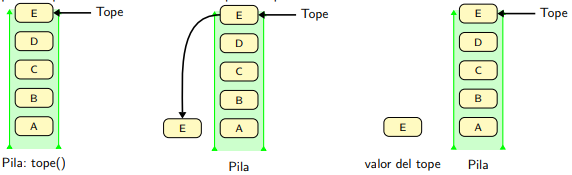
\includegraphics[width=0.8\textwidth]{diagrama1.png}
\caption{\label{fig:seq01}Ejemplo de un diagrama.}
\end{figure}


\begin{figure}[H]
\centering
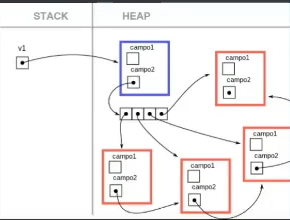
\includegraphics[width=0.8\textwidth]{diagrama2.png}
\caption{\label{fig:seq02}Otro ejemplo de un diagrama.}
\end{figure}


\end{document}
